\begin{center}
    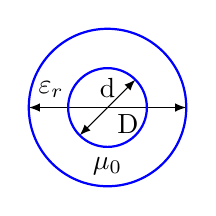
\begin{tikzpicture}
        \draw[latex-latex](-1,0)node[above right]{$\varepsilon_r$}--(1,0);
        \node[below right, yshift=1pt]{D};
        \draw[latex-latex, rotate=45](-0.5,0)--(.5,0);
        \node at (0,0)[above]{d};
        \draw[-, thick, blue](0,0) circle (1);
        \node at(0,-.75)[]{$\mu_0$};
        \draw[-, thick, blue](0,0) circle (0.5) ;
    \end{tikzpicture}


    D = Außendurchmesser

    d = Innendurchmesser
\end{center}
\vspace{-1em}
